\chapter{Background}

The impacts of global change are everpresent. Forest fires, hurricanes, and other extreme weather events...


In this ``global'' scale introduction, we should introduce the context of global change and the need for improved sensing and modeling to provide actionable insights at a pace that meets societal/human needs. We can then discuss how big data + machine learning can help fill in the gaps where our theoretical knowledge is incomplete, expensive (money an computational) to simulate directly, or plagued by initial condition sensitivity (e.g. Chaos).

Finish with a transition paragraph providing an overview of each of the following chapters

%% For Water Quality:
%% \begin{itemize}
%% \item chemical quantification (crude oil, algal blooms, terrorist events, etc...)
%% \item chemical identification (can we identify new constituents in the water?)
%% \end{itemize}

%% Outdoor Air Quality:
%% \begin{itemize}
%% \item How can we model the uncertainty of low cost sensors for real-time applications. This will have applications on real-time decision making, calibration, QA/QC, etc...
%% \item Can we leverage data to effectively model the dynamics of local air quality without the need for complicated microphysics simulations? (We can say something here about the need to go beyond thermodynamic equilibrium)
%% \item Can we learned models provide new insights into real physics? E.g. what do the learned terms of our SciML extended HAVOK model tell us? How can we interpret the forcing function? What do the learned coordinates of the HNN represent? How can we interpret dynamics on the Hamiltonian surface?
%% \end{itemize}


%% Indoor Air Quality:
%% \begin{itemize}
%% \item Can we leverage cutting edge measurement techniques to effectively model indoor chemical kinetics?
%% \item What is the role of ion chemistry in indoor air quality?
%% \item By combining observed species concentrations with highly detailed kinetics, can we infer the presence and role of species below detectable limits?
%% \end{itemize}

%% For the proposal, let's end the introduction with a timeline (we can use Dr. Lary's Gantt chart).


%% \section{Global Change}

%% Global change refers to the significant and long-term alterations in the Earth's physical, chemical, and biological systems, resulting from natural and human-induced processes \cite{IPCC2014, IPCC2018, UN2015}. This includes changes in the climate, land use, biodiversity, and biogeochemical cycles, as well as interactions among these systems. Global change can have profound impacts on natural and human systems, including altered weather patterns, sea level rise, increased frequency and severity of extreme events, loss of biodiversity and ecosystem services, and effects on human health and well-being. Understanding and managing global change is a critical challenge facing society today, requiring interdisciplinary approaches and collaboration across sectors and regions.

%% Global change can have a range of impacts on society, including environmental, social, and economic effects. Some of the aspects of global change that have the biggest impact on society include:

%% \begin{itemize}
%% \item Climate Change: Climate change, driven by human activities such as burning fossil fuels, deforestation, and land-use changes, has impacts on natural systems such as ocean acidification, sea level rise, and changes in precipitation patterns. These impacts can have cascading effects on human systems, including impacts on food security, water availability, and health.
%% \item Biodiversity Loss: Global change can lead to the loss of biodiversity, which can have impacts on ecosystem functioning and services, such as pollination, pest control, and carbon storage. These impacts can have indirect effects on human well-being, including impacts on food security, health, and cultural heritage.
%% \item Land Use Change: Land use change, such as deforestation, urbanization, and agriculture, can have impacts on natural systems such as soil quality, water availability, and biodiversity. These impacts can have direct and indirect effects on human systems, including impacts on food security, water availability, and cultural heritage.
%% \item Economic and Social Inequality: Global change can exacerbate economic and social inequality, with impacts on access to resources, health, and well-being. These impacts can have cascading effects on the ability of societies to adapt and respond to global change.
%% \item Human Health: Global change can have significant impacts on human health \cite{WHO2018, Costello2009, Haines2006}, both directly and indirectly, for example:
%%   \begin{itemize}
%%   \item Heat-related Illness: As temperatures increase due to global warming, there is an increased risk of heat-related illness, including heat exhaustion and heat stroke, particularly in vulnerable populations such as the elderly, young children, and outdoor workers.
%%   \item Air Pollution: Global change can lead to increased air pollution, including from sources such as wildfires and fossil fuel combustion. Exposure to air pollution can increase the risk of respiratory and cardiovascular diseases, including asthma, chronic obstructive pulmonary disease (COPD), and heart disease.
%%   \item Vector-borne Diseases: Changes in temperature and precipitation patterns can affect the distribution and abundance of disease vectors such as mosquitoes and ticks, leading to increased risks of vector-borne diseases such as dengue fever, malaria, and Lyme disease.
%%   \item Waterborne Diseases: Changes in precipitation patterns and water quality can increase the risk of waterborne diseases, including cholera and other diarrheal diseases.
%%   \item Food Security: Global change can affect food production and availability, leading to food shortages and malnutrition, particularly in vulnerable populations such as children and pregnant women.
%%   \end{itemize}
%% \end{itemize}

%% Effectively addressing these aspects of global change requires interdisciplinary approaches and collaboration across sectors and regions, as well as a commitment to sustainable development and equitable solutions. Adaptation and mitigation are two strategies for addressing global change, which differ in their focus and approach.

%% Adaptation involves taking measures to adjust and respond to the impacts of global change that are already occurring or are expected to occur in the future. This can include actions such as building sea walls to protect against sea level rise, developing drought-resistant crops, and improving public health infrastructure to address the increased risk of vector-borne diseases. Adaptation strategies aim to reduce the vulnerability of human and natural systems to the impacts of global change and increase their resilience.

%% Mitigation involves taking measures to reduce the drivers of global change, such as greenhouse gas emissions, land use change, and deforestation. This can include actions such as increasing energy efficiency, shifting to renewable energy sources, and reducing waste and consumption. Mitigation strategies aim to address the root causes of global change and reduce its severity and impact.

%% Both adaptation and mitigation are important strategies for addressing global change, but they differ in their focus and approach. Adaptation strategies focus on responding to the impacts of global change that are already occurring or are expected to occur in the future, while mitigation strategies focus on reducing the drivers of global change and preventing its impacts from occurring in the first place. A comprehensive approach to global change will require both adaptation and mitigation strategies, as well as efforts to promote sustainable development and equitable solutions.




%% \section{The Role of Sensing}

%% Sensing technologies can play a critical role in both adaptation and mitigation efforts by providing data and information that can inform decision-making and improve the effectiveness of strategies \cite{UNEP2017, NRC2010, CEN2017}.

%% In adaptation efforts, sensing technologies can provide real-time data on environmental conditions such as temperature, precipitation, sea level, air quality, as well as on the status and health of ecosystems and wildlife. This information can be used to inform early warning systems for natural disasters, to track the spread of vector-borne diseases, and to monitor the impacts of climate change on biodiversity and ecosystem services. Sensing technologies can also provide data on the effectiveness of adaptation measures, such as the performance of sea walls and other infrastructure.

%% In mitigation efforts, sensing technologies can provide data on greenhouse gas emissions and other drivers of global change, as well as on the effectiveness of mitigation measures such as renewable energy and carbon capture and storage. Sensing technologies can also be used to monitor and manage land use changes such as deforestation and urbanization, and to track the impacts of these changes on ecosystems and carbon storage.

%% Overall, sensing technologies can provide critical data and information for both adaptation and mitigation efforts, helping to improve decision-making and increase the effectiveness of strategies. The integration of sensing technologies with other tools such as modeling and data analysis can also help to identify new strategies and solutions for addressing global change. There are various sensing technologies and approaches used for monitoring the global environment. Here are some of the key ones:
%% \begin{itemize}
%% \item Remote Sensing: This technology involves using satellites and other airborne platforms to collect data on the Earth's atmosphere, land, and oceans. Remote sensing provides information on environmental parameters such as temperature, humidity, air quality, land use and land cover, and ocean temperature, salinity, and sea level \cite{Thenkabail2019, Buyantuyev2017, Gamon2016, Wang2017, Pasher2019}. Some examples of remote sensing include:
%%   \begin{itemize}
%%     \item Lidar: This technology uses laser pulses to measure distance and can be used to create detailed three-dimensional maps of the environment. Lidar is commonly used to measure forest canopy height, but can also be used to measure atmospheric conditions such as cloud cover and aerosol concentrations.
%%     \item Imaging Spectroscopy: This technology uses a combination of imaging and spectroscopy to measure the reflectance of different wavelengths of light. Imaging spectroscopy can be used to identify and map different types of vegetation and minerals, and can provide information on the health of plant communities.
%%     \item Unmanned Aerial Vehicles (UAVs): These are remote-controlled or autonomous aircraft that can be equipped with sensors for remote and in-situ  environmental monitoring. UAVs can be used for mapping and monitoring of large areas, and can collect high-resolution data on environmental conditions.
%%   \end{itemize}
%% \item In-Situ Sensors: These sensors are used to collect data directly from the environment at the location of interest. They can measure environmental parameters such as temperature, pressure, and humidity, as well as water quality and soil moisture. In situ sensors are commonly used in marine environments to measure ocean temperature, salinity, and other properties. Some examples of in-situ sensing include:
%%   \begin{itemize}
%%   \item Weather Stations: These are automated weather monitoring systems that collect data on atmospheric conditions such as temperature, humidity, barometric pressure, wind speed and direction, and precipitation. Weather stations can be installed on land or in the ocean to provide continuous monitoring of environmental conditions.
%%   \item Ground-Based Sensors: These sensors are used to monitor the quality of air, water, and soil. They can detect and measure pollutants such as carbon dioxide, nitrogen dioxide, ozone, sulfur dioxide, and particulate matter. Ground-based sensors are installed in various locations such as cities, industrial sites, and rural areas to provide localized environmental monitoring.
%%   \item Acoustic Sensors: These sensors are used to monitor environmental noise levels, including noise from traffic, industrial sources, and natural sources such as wind and waves. Acoustic sensors can provide information on noise levels over time and across different locations.
%%   \end{itemize}
%% \end{itemize}

%% Overall, these sensing technologies play a critical role in monitoring the global environment and can provide valuable information for environmental research, management, and policy-making.

%% \section{The Role of Computational Modelling}

%% Computer modeling can play a valuable role in both understanding and predicting global change \cite{Chen2019, Hantson2016, DeLucia2021, Oleson2013, Clark2016}. For example:
%% \begin{itemize}
%% \item Climate Modeling: Computer models can be used to simulate the Earth's climate system and predict future climate conditions. These models can incorporate data on greenhouse gas emissions, land use changes, and other factors to project how the Earth's climate will change over time.
%% \item Ecosystem Modeling: Computer models can be used to simulate how ecosystems will respond to changes in environmental conditions, such as changes in temperature, precipitation, and atmospheric composition. These models can help predict how changes in ecosystems will impact biodiversity, ecosystem services, and human well-being.
%% \item Carbon Cycle Modeling: Computer models can be used to simulate the global carbon cycle, which is the exchange of carbon between the Earth's atmosphere, land, and oceans. These models can help predict how changes in carbon emissions and land use will impact atmospheric carbon dioxide concentrations and global climate.
%% \item Air Quality Modeling: Computer models can be used to simulate air quality, including the dispersion of pollutants in the atmosphere. These models can help predict how changes in emissions and atmospheric conditions will impact air quality and human health.
%% \item Hydrological Modeling: Computer models can be used to simulate the movement of water through the Earth's hydrological cycle. These models can help predict how changes in precipitation, land use, and other factors will impact water availability, quality, and distribution.
%% \end{itemize}

%% Overall, computer modeling can provide valuable insights into the complex processes and interactions that drive global change. These insights can inform policy decisions and help guide efforts to mitigate and adapt to the impacts of global change.


%% \section{Key Technologies}


%% \subsection{Julia for Scientific Computing}

%% Julia is designed to combine the ease of use and high-level abstractions of languages like Python with the performance of compiled languages like C++, achieving a unique combination of speed and productivity for numerical and scientific computing.  Julia is a high-level, high-performance programming language designed for numerical and scientific computing. It combines the ease of use and readability of Python with the speed and efficiency of Fortran or C.   Julia has a wide array of scientific computing functionality, making it a powerful language for numerical analysis, data science, and engineering. It has built-in support for arrays and linear algebra, as well as packages for differential equations, optimization, probabilistic programming, data analysis and visualization, parallel and distributed computing, and machine learning. Julia's combination of performance, expressiveness, and flexibility make it an excellent choice for scientific and engineering applications, allowing for high-level abstractions and rapid prototyping, while still providing low-level control and efficient execution.

%% Here are some examples of what can be done easily in Julia that may not be as easy or efficient in other widely used scientific computing languages such as Python or Fortran:
%% \begin{itemize}
%% \item Multiple dispatch: Julia has a powerful multiple dispatch system that allows for generic programming and efficient function overloading. This allows for more flexible and expressive code compared to traditional object-oriented programming (OOP) in Python. Multiple dispatch allows a function to behave differently based on the types and/or number of arguments passed to it. In other words, the behavior of a function can be dispatched based on the specific types and/or number of arguments passed to it.
%% \item Just-in-time (JIT) compilation: Julia's JIT compiler translates high-level Julia code into optimized machine code, making Julia programs run nearly as fast as C or Fortran. In contrast, Python code is interpreted, and Fortran requires pre-compilation.
%% \item Distributed computing: Julia has built-in support for distributed computing, making it easy to parallelize and scale up computations across multiple processors or machines. This is not as easy to do in Python or Fortran.
%% \item Units and Error Propagation: The Units package in Julia provides a powerful and flexible framework for handling physical units in computations, useful for error propagation and dimensional analysis, helping to ensure that the results are accurate, consistent, easy to interpret, and dimensionally consistent.
%% \item Built-in unit testing: Julia has a built-in testing framework that makes it easy to write and run unit tests for your code, ensuring that it works correctly.
%% \item ISO characters: Julia supports the use of Greek and other ISO characters in variable and function names, which can make code more readable and expressive, especially in mathematical or scientific contexts.
%% \item Interactive data visualization: Julia has a number of powerful data visualization packages, such as Plots.jl and Makie.jl, that allow for interactive, high-performance data visualization.
%% \item Package management: Julia has a sophisticated package manager that makes it easy to install, manage, and use third-party packages in your code. This is not as easy to do in Fortran, and while Python has a package manager, Julia's package manager is faster and more reliable.
%% \item Inline C/Fortran/Python/R/Matlab code: Julia allows for inline C, Fortran, Python, R or Matlab code, making it easy to use existing libraries and code written in these languages without having to rewrite everything in Julia.
%% \end{itemize}


%% \subsection{Scientific and Physics-based Machine Learning}

%% Scientific machine learning (SciML) refers to the application of Machine Learning (ML) techniques to scientific problems, where the goal is not only to make predictions but also to gain insights into the underlying physical processes \cite{raissi2019physics, rackauckas2020universal, carleo2019machine}. SciML involves the integration of domain-specific knowledge and physical models with data-driven techniques, and it has the potential to revolutionize many areas of science and engineering. In this thesis we explore the use of Physics-based machine learning (PBML) \cite{Raissi2021, Wu2021} for a variety of applications.

%% Recent examples include a paper by \cite{raissi2019physics} that introduces a physics-informed neural network (PINN) framework for solving nonlinear partial differential equations, a paper by \cite{rackauckas2020universal} that proposes a universal differential equation (UDE) approach to scientific machine learning, and a review article by \cite{carleo2019machine} that discusses the use of machine learning in various fields of physics, including condensed matter physics, high-energy physics, and quantum physics. PBML has several advantages over purely data-driven approaches, including:

%% \begin{itemize}
%% \item Improved generalization: PBML models incorporate prior knowledge of the underlying physics, resulting in models that are more interpretable and generalizable. This enables the models to make accurate predictions even with limited training data.
%% \item Incorporation of physical constraints: PBML models can be designed to incorporate physical constraints, such as conservation laws, which can help to ensure physically consistent predictions.
%% \item Improved interpretability: PBML models are more interpretable than purely data-driven models since they are designed to incorporate physical principles. This can enable scientists and engineers to gain deeper insights into the underlying mechanisms of the systems they are studying.
%% \item Reduced data requirements: PBML models require less training data than purely data-driven models since they leverage the physics-based priors, reducing the need for large datasets to train accurate models.
%% \item Better extrapolation: PBML models are better equipped to extrapolate beyond the training data since they incorporate knowledge of the underlying physics, enabling them to make more accurate predictions in new and unseen scenarios.
%% \end{itemize}

%% Overall, PBML has several advantages over purely data-driven approaches, including improved generalization, reduced data requirements, better extrapolation, incorporation of physical constraints, and improved interpretability, making it a valuable tool for scientific and engineering applications.



%% \textcolor{red}{NOTE: We should combine chapter on Physical Context with this one}

%% We should end with some comments on work complete and work proposed as well as a tentative schedule




\section{Water Quality}

\subsection{Properties of Aqueous Solutions}
\subsection{Reflectance Spectroscopy}

\textcolor{red}{NEEDS UPDATING/REWORDING:}

The quantitative description of light absorption by a sample is based on the Beer-Lambert (or, more correctly, Beer-Lambert-Bouger) law. In deriving this law, we consider that incident monochromatic light of intensity I0 crosses an infinitesimal thickness, dl, of an absorbing species of concentration c. The decrease in light intensity, dI, is proportional to the thickness of the sample, the concentration of the absorbing species and the incident light intensity

\begin{equation}
dI = -a(\lambda)CI d\ell
\end{equation}
so that upon integrating, we find
\begin{equation}
  I(\lambda) = I_0(\lambda)\exp(-a(\lambda)C\ell)
\end{equation}


\subsection{Solar Geometry}

An explanation of relevant solar angles as well as their determination (i.e. the code I ported to Julia from Matlab script Dr. Lary supplied). We should also comment on the importance of

Use David's figure from his book to illustrate the solar geometry.



\section{Air Quality}

Exposure to air pollution has been linked to a wide range of health effects \cite{Brook2008, Kelly2011, Xu2017}, including respiratory and cardiovascular diseases, cancer, and adverse birth outcomes. Further, physical sensing provides valuable data and the basis for international assessments such as the Intergovernmental Panel on Climate Change (IPCC), which seeks to assess the science related to climate change and its impacts on natural and human systems \cite{IPCC1990, IPCC1995, IPCC2001, IPCC2007a, IPCC2007b, IPCC2007c, IPCC2013a, IPCC2013b, IPCC2014, IPCC2018, Friedlingstein2020, Huang2017}.

\subsection{Pollution and Particulate Matter}
discuss sources, evolution, global trends, etc...

\subsection{Indoor Air Quality}

This statement serves as the foundation for The Clean Air in Buildings Challenge and this RFI. We completely agree with this premise, but we believe the ‘order of operations’ - among ventilation, filtration, and air cleaning - should be the primary focus of inquiry, and effective and safe air cleaning innovations should be a focus deserving full consideration. We can reconcile multiple, often competing goals by informing and empowering schools and commercial buildings to adopt a  Clean First mentality, which we will explore in this response, as well as examine the ‘art of the possible’ by taking a critical look at the $21^{st}$ century innovations we believe will be essential to the practical pursuit and achievement of The Clean Air in Buildings Challenge goals/objectives. We will demonstrate the necessary considerations of a Clean First approach as well as highlight its additional benefits in this response, which include but are not limited to:


\begin{itemize}
\item Reduced mechanical system energy consumption.
\item Reductions in healthcare-acquired infections (HAIs) that are statistically significant in healthcare settings.
\item Real-world testing/proof of lower microbiological burden (total and culturable bacteria, fungi, and their spores) in addition to improved ventilation/filtration alone.
\item Reduced school absenteeism.
\item Increased resiliency to future pandemics and communicable diseases.
\item Reduction in airborne communicable disease and allergen loads.
\end{itemize}


The real challenges posed by global environmental change, combined with rising utility costs as a result of inflation and geopolitical shocks to energy supply chains, have created an implicit dichotomy between climate and public health goals. As Prof. Bahnfleth has said,



\section{Physics of Chemical Reactions: Chemical Reaction Kinetics}

\subsection{Overview}

Since the early successes of Newton's descriptions of mechanics by means of simple forces acting on masses, scientists have sought to understand the dynamics of chemical reactions in terms of the detailed microphysics of molecular collisions. As we shall see, this approach can be utilized productively to justify the complicated temperature and pressure dependence of the reaction rate coefficients of many elementary reaction. However, even when considering the asymmetric structure of many molecules, and therefore, the dependence on orientation at the collision site, kinetic theory alone is unable to model reaction rates in all relevant temperature and pressure regimes. To do this, one can utilize the modern treatment of \textit{Potential Energy Surface} (PES) theory together with the notion of short-lived, unstable intermediate reaction states to calculate reaction rate coefficient functions for specific reactants. \textit{Ab initio} solution of the Schrodinger equation for the relevant nuclear geometries ($3N$ reaction coordinates for $N$ atoms) together with scattering and spectroscopic methods as suggested by \cite{transition-state-spectroscopy-bimol} have led to significant improvements in our understanding of reaction dynamics.



\begin{figure}[h]
  \centering
  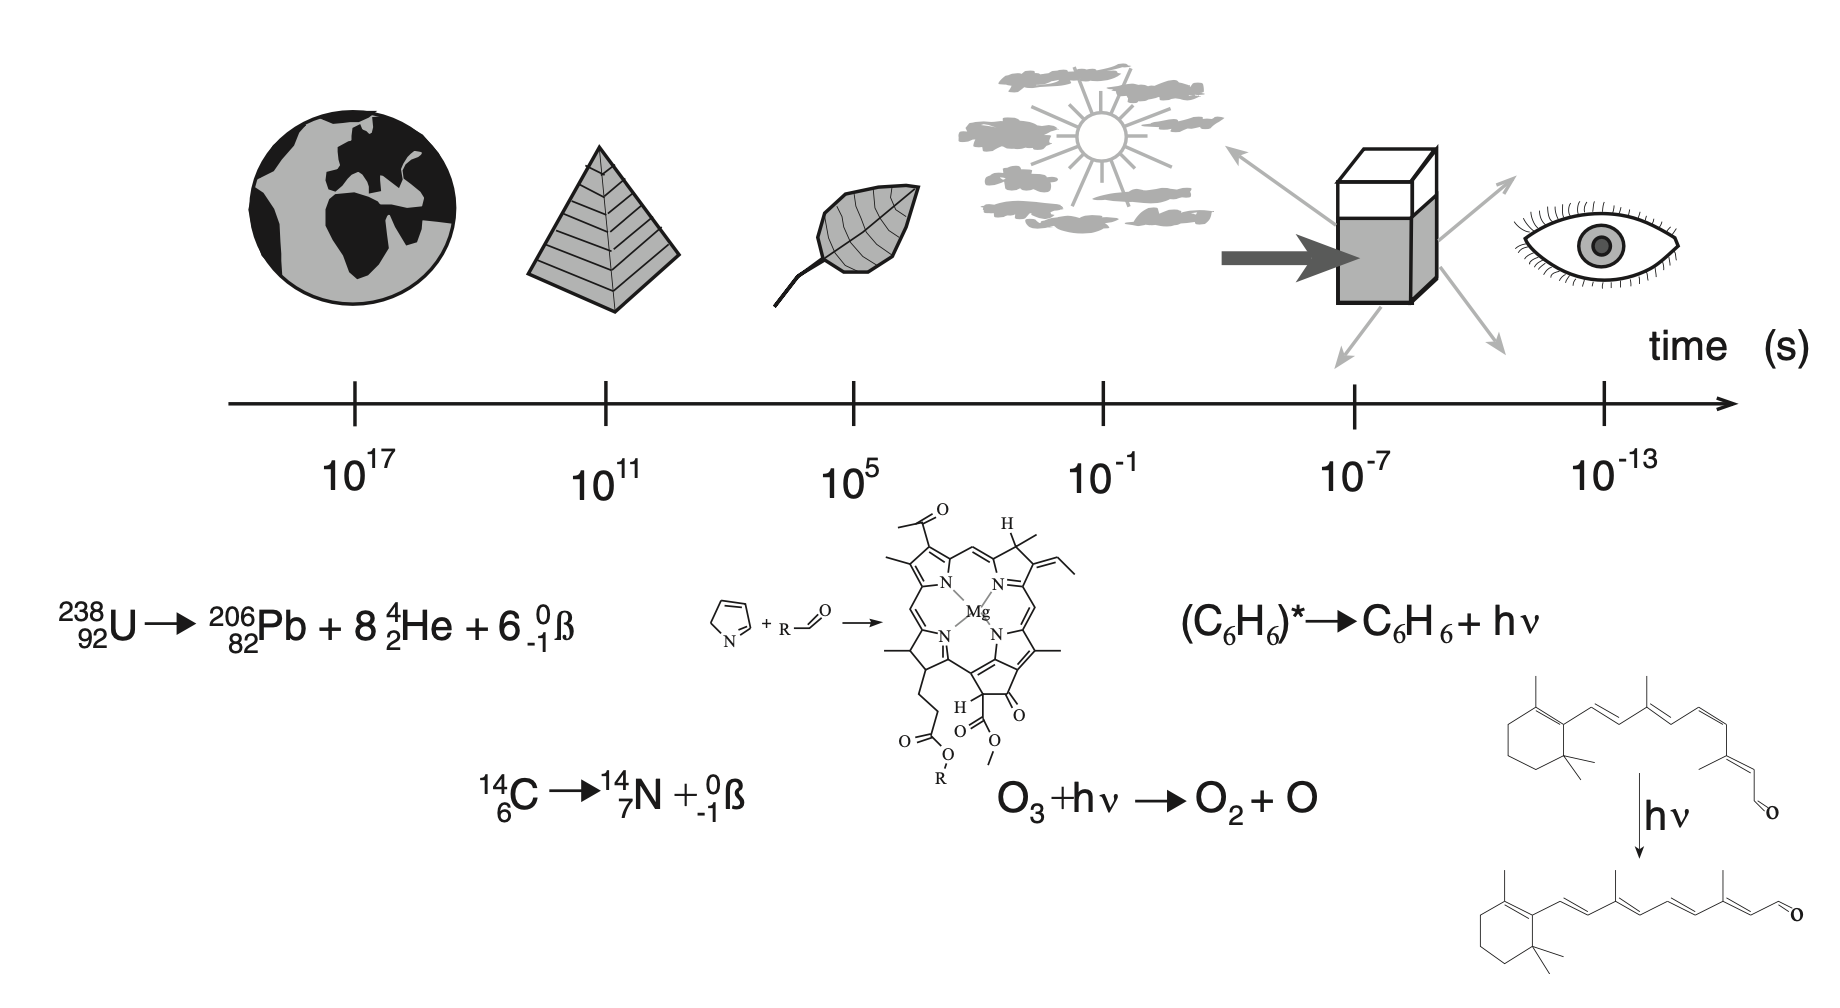
\includegraphics[width=0.85\textwidth]{introduction/reaction-timescales.png}
  \caption{An illustration of the broad range of reaction time scales from the long-lived nuclear decay to rapid degradation of molecules by photolysis. Figure taken from \cite{arnaut2006chemical}}
  \label{fig:reaction-timescales}
\end{figure}


However the computational complexity of this task makes it prohibitively expensive to perform at the scale required for our desired chemical mechanism which consists of many hundreds to thousands of reactants together with as many as 16,000 unique reactions. Therefore in the following discussion, we shall primarily utilize the kinetic theory to justify the functional form for \textit{most} rate coefficients with some reference to the extensions made by PES theory. We note that in practice, kinetic evaluations such as the periodic reports from the NASA Jet Propulsion Laboratory \cite{jpl-kinetic-evaluation-2020} utilize (justified) empirical fits to provide suggested functional forms for reaction rate coefficients.

\subsection{Chemical Equilibrium and the Law of Mass Action}

Before outlining the dynamics involved during complex chains of chemical reactions, it is worth spending some time to consider how we should treat chemical equilibrium. Usually in these scenarios we can not hold the internal energy fixed due to interactions with the environment, but rather, the temperature and pressure can often be treated as so. For example, we may be interested in gas-phase reactions occurring in ambient indoor air at or near standard temperature and pressure. In such scenarios, one finds the relevant potential energy to be the Gibbs, given by
\begin{equation}
  G = U - TS + PV,
\end{equation}
which is minimized in equilibrium under constant temperature and pressure.

This equation leads to the convenient thermodynamic identity
\begin{equation}
  dG = -SdT + VdP + \sum_i \mu_i dN_i
\end{equation}
from which we may identify the \textit{chemical potential} of the $i^{th}$ species as
\begin{equation}
  \mu_i  = \left(\frac{\partial G}{\partial N_i} \right)_{T,P,N_{j\neq i}}.
\end{equation}
The fact that each $\mu_i$ depends only on intensive state variables allows us to further simplify the relationship by considering what would happen were we to gradually increase the size of the system while maintaining the values of intensive parameters $T$, $P$, $\mu_i$. The result is G must increase in direct proportion to the increase in each $N_i$, that is:
\begin{equation}
  \label{eq:free-energy-definition}
  G = \sum_i \mu_i N_i.
\end{equation}
From equation \ref{eq:free-energy-definition} it is clear that the $\mu_i$ can be understood as molecular \textit{potentials} (i.e. chemical energy per molecule) in analogy to the notion of electric potential as a energy per unit charge.


For an ideal gas consisting of a single component we can combine equation \ref{eq:free-energy-definition} together with the identity
\begin{equation}
  V = \left(\frac{\partial G}{\partial P}\right)_{T,N}
\end{equation}
to obtain
\begin{equation}
  \left(\frac{\partial \mu}{\partial P}\right)_{T,N} = \left(\frac{\partial}{\partial P}\frac{G}{N}\right)_{T,N} = \frac{1}{N}\left(\frac{\partial G}{\partial P} \right)_{T,N} = \frac{V}{N} = \frac{kT}{P}
\end{equation}
so that by integration from a reference pressure, say $P_0= 1$ atm, we obtain the handy expression for the chemical potential
\begin{equation}
  \label{eq:mu-ideal}
  \mu(T,P) = \mu(T,P_0) + kT\ln(P/P_0)
\end{equation}
which we shall use again momentarily.

%% To understand what happens to $G$ at equilibrium where we know $dG=0$, let's now consider a homogeneous dilute mixture of a chemical species $B$ into species $A$. In the absence of $B$, we should have
%% \begin{equation}
%%   \label{eq:gibbs-A}
%%   G = N_{A}\mu_{0}(T,P)
%% \end{equation}
%% where $\mu_0$ denotes the chemical potential of the pure substance with just $A$. Adding a single particle of $N_{B}$ would then lead to an increase in free energy by some intrinsic amount $f(T,P)$ in addition to an increase from the added entropy due to the fact that we can place the particle (to a reasonable approximation) near anyone of the $N_{A}$ original particles. Therefore, we should expect an increase of
%% \begin{equation}
%%   dG = f(T,P) -T(k\ln(N_{A}))
%% \end{equation}

%% If we continue to add more particles until $N_{B}$, we will have added a total of $N_{B}$ contributions of $f(T,P)$ in addition to an entropy increase from an added multiplicity of states amounting to $N_{A}^{N_{B}}/N_{B}!$ or,
%% \begin{equation}
%%   \begin{aligned}
%%     dG &= N_{B}f(T,P) - N_{B}kT\ln(N_{A}) + kT\ln(N_{B}!) \\
%%     &\approx N_{B}f(T,P) - N_{B}kT\ln(N_{A}) + kTN_{B}(\ln(N_{B})-1) \qquad\text{(Stirling)}
%%     \end{aligned}
%% \end{equation}
%% putting this together with equation \ref{eq:gibbs-A}, we obtain
%% \begin{equation}
%%   G = N_{A}\mu_0(T,P) + N_{B}f(T,P) - N_{B}kT\ln(N_{A}) + N_{B}kT\ln(N_{B}) - N_{B}kT
%% \end{equation}

Returning now to the notion of chemical equilibrium, recall that we must have $dG=0$ so that $G$ is minimized. At constant temperature and pressure, this means
\begin{equation}
  0 = dG = -\cancel{SdT} + \cancel{VdP} + \sum_i \mu_i dN_i = \sum_i\mu_i dN_i
\end{equation}
and therefore, a generic reaction of the form
\begin{equation}
  \nu_1X_1 + \nu_2X_2 + \cdots \leftrightarrow \nu_3 X_3 + \nu_4 X_4 \cdots
\end{equation}
with chemical species $X_i$ and stoichiometric coefficients $\nu_i$ satisfies the condition that
\begin{equation}
  \nu_1\mu_1 + \nu_2\mu_2 + \cdots = \nu_3\mu_3 + \nu_4\mu_4 + \cdots.
\end{equation}

If we now make use of equation \ref{eq:mu-ideal} with the identification of $\mu^0 = \mu(T,P_0)$, then we obtain
\begin{equation}
  \sum_{i}^{\text{products}}\nu_i\mu_i^0 + \nu_i kT\ln(P_i/P_0) = \sum_{j}^{\text{reactants}} \nu_j\mu_j^0 + \nu_j kT\ln(P_j/P_0).
\end{equation}
collecting terms involving the $\mu^0_k$ to one side and multiplying through by Avogadro's constant, we obtain
\begin{equation}
  RT\ln\left(\frac{\prod\limits_j^{\text{reactants}}\left(\frac{P_i}{P_0}\right)^{\nu_i}}{\prod\limits_j^{\text{products}}\left(\frac{P_j}{P_0}\right)^{\nu_j}}\right) = R\left(\sum_j^{\text{reactants}}\nu_j\mu_j^0 -  \sum_i^{\text{products}} \nu_i\mu_i^0\right) = \Delta G^0
\end{equation}
so that by exponentiation, we arrive at the simple expression:
\begin{equation}
  \frac{\prod\limits_j^{\text{products}}\left(\frac{P_j}{P_0}\right)^{\nu_j}}{\prod\limits_i^{\text{reactants}}\left(\frac{P_i}{P_0}\right)^{\nu_i}} = \exp(-\Delta G^0/RT)
\end{equation}
which through further application of the ideal gas law yields
\begin{equation}
  \label{eq:law-of-mass-action}
  \boxed{\frac{\prod\limits_j^{\text{products}}\left(X_j\right)^{\nu_j}}{\prod\limits_i^{\text{reactants}}\left(X_i\right)^{\nu_i}} = K_{\text{eq}}}
\end{equation}
Here $K_{\text{eq}}$ is a temperature dependent constant called the \textit{equilibrium constant} for the reaction, and equation \ref{eq:law-of-mass-action} is called the \textit{law of mass action}. This expression indicates what we can expect to find if we allow our reactive system to proceed far enough to reach equilibrium. We shall later utilize this expression to perform a thermodynamic \textit{sanity check} as is described in \cite{boldi-thesis}. 


\subsection{Reaction Rate Laws}

Having established the expected behavior at equilibrium, our task now is to establish the correct dynamical laws describing the variety of reactions which take place. To begin, let us consider again a generic chemical reaction of the form
\begin{equation}
  \nu_{1}X_1 + \nu_{2}X_2 + \cdots \longrightarrow \nu_{3}X_3 + \nu_{4}X_4 + \cdots
\end{equation}

To describe the dynamical process of a reaction, we can introduce a parameter $\xi$ called the \textit{reaction extent} such that at any time we have
\begin{equation}
  \xi(t) = \frac{\lvert N_i(t) - N_i(0) \rvert}{ \nu_i}
\end{equation}
where $N_i(t)$ is the number  of the $i^{th}$ species and $\nu_i$ is the stoichiometric coefficient. The reaction rate is then easily understood as the rate of change of the reaction extent,
\begin{equation}
  r := \frac{d\xi}{dt} = \frac{1}{\nu_i}\left\lvert \frac{dN_i(t)} { dt} \right\rvert.
\end{equation}
Manipulating this expression to introduce the volume then leads us to
\begin{equation}
  r(t) = \frac{1}{\nu_i}\left\lvert\frac{dN_i}{dt}\frac{V}{V} \right\rvert = \frac{V}{\nu_i}\left\lvert \frac{d[X_i]}{dt} \right\rvert
\end{equation}
where $[X_i]$ denotes the concentration (number density) of the $i^{th}$ species participating in the reaction. All this is to say that upon rearranging the expression, we find
\begin{equation}
  \left\lvert \frac{d[X_i]}{dt} \right\rvert = \nu_i\frac{r(t)}{V} = \nu_iv,
\end{equation}
or in words, the absolute change in concentration of the $i^{th}$ species as a function of time is proportional the quantity $v=r(t)/V$ (called the reaction \textit{velocity}) scaled by the stoichiometric coefficient $\nu_i$ of the $i^{th}$ species. For the purposes of our modeling tasks, we must now establish appropriate forms for the reaction velocity in terms of the relevant thermodynamic variables (i.e. temperature, and pressure) and constituent concentrations.

To begin, let us consider a bimolecular reaction
\begin{equation}
  A + B \longrightarrow \text{Products}.
\end{equation}
The simplest approach to modeling the reaction velocity for reactions of this type is to make the assumption that \textit{each molecular collision leads to a reaction}. From this perspective, should then be able to derive the reaction velocity using the established statistics of molecular velocities together with appropriate data for the size of each reactant.

Let us treat reacting species as \textit{hard spheres} of radii $r_{A}$ and $r_{B}$ respectively, or in other words, the molecules are spheres which only interact by contact (no long range interactions). Then a collision will occurs if the separation $d_{AB}$ satisfies
\begin{equation}
  d_{AB} = r_{A} + r_{B}
\end{equation}

\textcolor{red}{NOTE: Add image of hard spheres here}

To start, let's consider collisions where $B$ are stationary and $A$ is seen to move with velocity $\mathbf{v}_{A}$.

\textcolor{red}{NOTE: Add image of hard spheres forming cylinder here}

Then during a time $dt$, the molecule $A$ sweeps out a cylindrical volume
\begin{equation}
  dV = \pi d_{AB}^2 v_{A}dt
\end{equation}
in which collisions may occur. Supposing we have a density $N_{B}/V$ of species $B$, then the collision rate (collisions per second) for a single particle of $A$ will be
\begin{equation}
  \frac{dV}{dt}\frac{N_{B}}{V} = \frac{\pi d_{AB}^2 v_{A}N_{B}}{V}
\end{equation}
and therefore, the reaction velocity for $N_{A}$ particles with average velocity $\overline{\mathbf{v}}_{A}$ is
\begin{equation}
  v = \frac{\pi d_{AB}^2 \overline{v}_{A}N_AN_B}{V^2}
\end{equation}

if instead particles of both $A$ and $B$ move relative to each other, then their \textit{relative} velocity is given by the law of cosines:
\begin{equation}
  v_{AB}^2 = v_{A}^2 + v_{B}^2 - 2v_{A}v_{B}\cos(\theta)
\end{equation}
which, since all directions are equally probable, yields an average relative velocity of
\begin{equation}
  \overline{v_{AB}}^2 = \sqrt{\overline{v_{A}}^2 + \overline{v_{B}}^2}.
\end{equation}

The relative velocity describes the motion of the reduced mass $\mu=m_{A}m_{B}/(m_{A}+m_{B})$ and therefore under the standard Maxwellian velocity distribution, leads to
\begin{equation}
  \overline{v_{AB}} = \sqrt{\frac{8kT}{\pi \mu}}
\end{equation}
Combining everything together yields the reaction velocity
\begin{equation}
  v = \pi d_{AB}^2\frac{N_{A}}{V}\frac{N_{B}}{V}\sqrt{\frac{8kT}{\pi \mu}} = \pi d_{AB}^2[A][B]\sqrt{\frac{8kT}{\pi \mu}}
\end{equation}
which we might further simplify as
\begin{align}
  v &= k[A][B] \\
  k &= \pi d_{AB}^2\sqrt{\frac{8kT}{\pi \mu}} = \sigma \sqrt{\frac{8k_BT}{\pi \mu}}
\end{align}
where $k$ is called the \textit{reaction rate coefficient} and $\sigma$ is the \textit{reaction cross section}.

Excellent! We have discovered a couple of key features for the reaction velocity, namely, that it depends on a polynomial combination of reactant concentrations, \textit{and} that there is clear temperature dependence due to the relationship between molecular velocities and temperature.

There are, however, some obvious limitations.
\begin{enumerate}
  \item Not all collisions occur with orientations favorable for reaction (i.e. the hard sphere model isn't realistic for species).
  \item Not all collisions will have enough enough energy for the reaction to proceed.
\end{enumerate}
These limitations were well known, and in particular, Arrhenius suggested a competing function based on empirical studies of with
\begin{equation}
  k = A\exp(-\alpha/T)
\end{equation}
where $\alpha$ is some constant that depends on the reaction taking place. We can address the first point in a \textit{hand-wavy} manner by simply including a geometric correction factor, $g\leq 1$, to account for the distribution of favorable orientations. To address the second point, it is worth establishing some minimal energy required for the reaction, $E_a$, by examining our Maxwellian distribution in closer detail. As we shall see, this will allow us to recover the exponential dependence suggested by Arrhenius.

The velocities $\mathbf{v}_{A}$ and $\mathbf{v}_{B}$ of each colliding pair of reactants define a plane. Therefore, for ease of calculation, we approximate the distribution of velocities near the collision site by the 2-dimensional Maxwellian speed distribution:
\begin{equation}
  f(v) = \frac{\mu}{k_BT}v\exp\left(-\frac{\mu v^2}{k_BT}\right)
\end{equation}
so that the fraction of particles with speed in the range $[v, v+dv]$ is
\begin{equation}
  \frac{dN(v)}{N_{tot}} = f(v)dv = \frac{\mu}{k_BT}v\exp\left(-\frac{\mu v^2}{k_BT}\right)dv.
\end{equation}
For an ideal gas under no external forces, we may identify the energy $\epsilon = \mu v^2/2$ so that $d\epsilon = \mu vdv$. Therefore, in energy space, this ratio becomes
\begin{equation}
  \frac{dN(\epsilon)}{N_{tot}} = \frac{1}{k_BT}\exp(-\epsilon/k_BT)d\epsilon
\end{equation}
If $E_a$ is the minimum (\textit{activation}) Energy required to engage the reactants, then the ratio of reactants with sufficient energy for the reaction to proceed is determined by integration to be
\begin{equation}
  \left.\frac{N(\epsilon)}{N_{tot}}\right\rvert_{\epsilon > E_{a}} = \int\limits_{\E_{a}}^{\infty}\frac{1}{k_BT}\exp(-\epsilon/k_BT)d\epsilon = \exp(-E_a/k_bT)
\end{equation}
so that we may justify an additional correction to our reaction rate coefficient
\begin{equation}
  k = g\pi d_{AB}^2\sqrt{\frac{8k_BT}{\pi \mu}}\exp(-E_{a}/k_BT)
\end{equation}

The final augmentation we can perform without before leaving collision theory behind is to observe that the cross-section $\sigma$ was treated independently from the requirement of a minimum activation energy. With that in mind, suppose instead that a reaction cross section \textit{only makes sense} if the reactants have the required minimum energy, that is
\begin{equation}
  \sigma(\epsilon) = \begin{cases}
    \pi d_{AB}^2 & \epsilon > E_{A} \\
    0 & \text{otherwise}
  \end{cases}
\end{equation}
If this is true, we can not keep the cross section outside of the ensemble average.

Allowing ourselves to utilize the full, three-dimensional Maxwellian speed distribution, we have
\begin{equation}
  \begin{aligned}
  k &= \int\limits_0^\infty \sigma(v)v f(v) dv \\
  &= 4\left(\frac{\mu}{2\pi k_BT} \right)^{3/2}\int\limits_0^\infty \sigma(v)v \cdot v^2\exp\left(-\frac{\mu v^2}{2k_BT} \right)dv
  \end{aligned}
\end{equation}
which in terms of energy yields
\begin{equation}
  \begin{aligned}
  k(T) &= \left(\frac{1}{\pi \mu} \right)^{1/2}\left(\frac{2}{k_BT}\right)^{3/2}\int\limits_{0}^{\infty}\epsilon\sigma(\epsilon)\exp(-\epsilon/k_BT)d\epsilon \\
  &= \left(\frac{1}{\pi \mu} \right)^{1/2}\left(\frac{2}{k_BT}\right)^{3/2}\int\limits_{E_a}^{\infty}\epsilon\pi d_{AB}^2\exp(-\epsilon/k_BT)d\epsilon \\
  &= \pi d_{AB}^2 \sqrt{\frac{8k_BT}{\pi \mu}}\left(1 + \frac{E_a}{k_BT} \right)\exp(-E_a/k_BT)
  \end{aligned}
\end{equation}

In summary, we have established that for bimolecular reactions, the (simple) theory of molecular collisions allows us to model the reaction velocity by
\begin{align}
  v &= k(T)[A][B] \\
  k(T) &\approx \pi d_{AB}^2 \sqrt{\frac{8k_BT}{\pi \mu}}\left(1 + \frac{E_a}{k_BT}\right)\exp(-E_a/k_BT)
\end{align}

To derive a more accurate form for the rate coefficient $k$, we can result to PES, simulation, and statistical sampling techniques \cite[for example]{pes-h-h2, pes-for-k}. For our purposes, it is enough to have justified the kinds of functional dependence on temperature we can expect to encounter when when collating available data on rate coefficients in the present literature.

\section{Photolysis}

Give an overview for photolysis (perhaps borrow from Dr. Lary's Textbook)

For experimental reasons, the wavelengths ($\lambda$) most commonly used for initiating photochemical processes vary between the ultraviolet ($200-250$ nm) and the near infrared ($750-800$ nm). Light at these wavelengths has an energy which corresponds roughly to $600-50 $ kJ $\text{mol}^{-1}$, which is very close to the energies of many chemical bonds.



\section{Summary of Chemical Mechanism Kinetics}

Give a summary of kinetics for each of the 3 reaction types. Then finish by writing the form of the combined differential equations for the entire system (and it's Jacobian)
